%==============================================================================
% Paper Research Methods: onderzoeksvoorstel specialisatie
%==============================================================================

\documentclass{hogent-article}

\usepackage{tikz}
\usetikzlibrary{positioning,arrows.meta}

\addbibresource{references.bib}

\studyprogramme{Professionele bachelor toegepaste informatica}
\course{Research Methods, 2A2}
\assignmenttype{Groepsopdracht}
\academicyear{2025-2026}
\title{Onderzoeksvoorstel: een geschikte webfilteroplossing voor het netwerk van College Ten Doorn}

\author{Sammy Karknawi} \email{sammy.karknawi@student.hogent.be}
\author{Lander Dhaen} \email{lander.dhaen@student.hogent.be}
\author{Nicolas Robinet} \email{nicolas.robinet@student.hogent.be}
\author{Tatjana Schouteeten} \email{tatjana.schouteeten@student.hogent.be}


\projectrepo{https://github.com/HoGentTIN/rm-25-26-groep-83}

\specialisation{System \& Network Engineering}
\keywords{DNS-filtering, contentfiltering, schoolnetwerk, DNS-over-HTTPS, vergelijkende studie, proof of concept}

\begin{document}

\begin{abstract}
    Dit onderzoeksvoorstel situeert zich binnen de specialisatie System \& Network Engineering en vertrekt vanuit een concrete casus: College Ten Doorn, een grote scholencampus in Eeklo, wil contentfiltering op haar schoolnetwerk sluitend afdwingen voor haar minderjarige leerlingen. Klassieke DNS-filtering wordt echter steeds makkelijker omzeild, onder meer door versleutelde DNS-protocollen. Via een vergelijkende studie met meetbare criteria en een proof of concept in een gevirtualiseerde testopstelling formuleren we een onderbouwde aanbeveling voor de meest geschikte filteroplossing voor deze school. De doelgroep van dit onderzoek zijn netwerkbeheerders van onderwijsinstellingen en kmo's met een gelijkaardige filterbehoefte.
\end{abstract}

\tableofcontents

\section{Probleemstelling}
College Ten Doorn is een grote katholieke scholencampus in Eeklo die onder meer secundair onderwijs aanbiedt aan enkele duizenden leerlingen. Leerlingen gebruiken het schoolnetwerk dagelijks met eigen of door de school beheerde laptops. De school heeft daarbij een zorgplicht: ze wil vermijden dat minderjarigen via haar infrastructuur toegang krijgen tot schadelijke of leeftijdsongeschikte content (bv. pornografie, gokwebsites, extremistische inhoud), en ze moet dit beleid ook technisch kunnen afdwingen.

Het kernprobleem is dat de huidige, beperkte filtering op het schoolnetwerk niet sluitend is en niet centraal geëvalueerd wordt. Klassieke filtering op basis van DNS is bovendien structureel onder druk komen te staan: versleutelde DNS-protocollen zoals DNS-over-HTTPS laten toe om DNS-verkeer buiten de filterende resolver om te sturen, waardoor netwerkfilters onzichtbaar gepasseerd worden \autocite{Hoffman2018}. Grootschalig meetonderzoek toont bovendien aan dat DNS-manipulatie als filtertechniek gekende beperkingen en omzeilingsroutes heeft \autocite{Pearce2017}. Ook in de Belgische context is bekend dat websiteblokkades op DNS-niveau eenvoudig te omzeilen zijn en juridisch zorgvuldig onderbouwd moeten worden \autocite{Royer2019}. Een school die filtert, moet daarnaast rekening houden met het spanningsveld met de vrijheid van meningsuiting en informatievergaring, wat een doordachte en proportionele technische keuze des te belangrijker maakt \autocite{Ombelet2015}.

Er bestaat een ruim aanbod aan filteroplossingen van open source (bv. Pi-hole, pfSense) tot commerciële clouddiensten (bv. Cisco Umbrella), maar er is geen pasklaar antwoord op de vraag welke oplossing voor déze school, met haar specifieke infrastructuur, budget en beheerscapaciteit, de beste keuze is. Dat is een typisch toegepast onderzoeksprobleem: de beste oplossing hangt af van de specifieke situatie en moet objectief, met meetbare criteria, bepaald worden.

\subsection{Doelgroep en relevantie}
De primaire doelgroep zijn de netwerkbeheerders van College Ten Doorn. De resultaten zijn daarnaast relevant voor IT-verantwoordelijken van andere onderwijsinstellingen en kmo's die contentfiltering willen invoeren of herevalueren. Meetplatformen zoals het Open Observatory of Network Interference tonen dat de effectiviteit van netwerkfilters wereldwijd een actueel onderzoeksthema is \autocite{OONI2026}.

\section{Hoofdonderzoeksvraag}
\begin{quote}
    Welke webfilteroplossing is het meest geschikt om het contentfilterbeleid van College Ten Doorn op haar schoolnetwerk af te dwingen, rekening houdend met haar infrastructuur, budget en beheerscapaciteit?
\end{quote}
Deze vraag is open (geen ja-neevraag), niet op te zoeken en niet in één stap te beantwoorden: ze vereist een analyse van de casus, een systematische vergelijking van alternatieven en een experimentele validatie.

\section{Deelvragen}

\subsection{Probleemdomein}
\begin{enumerate}
    \item Hoe zien de huidige netwerkinfrastructuur en het huidige filterbeleid van College Ten Doorn eruit, en waar schieten die tekort?
    \item Aan welke functionele en niet-functionele requirements moet een filteroplossing voor College Ten Doorn voldoen?
    \item Welke technieken voor webfiltering bestaan er (DNS-filtering, proxy-/TLS-inspectie, firewall-categorisatie) en wat zijn hun gekende beperkingen en omzeilingsmogelijkheden?
\end{enumerate}
Relevante bronnen voor het probleemdomein zijn onder meer \textcite{Pearce2017} over de werking en beperkingen van DNS-manipulatie, \textcite{Hoffman2018} over versleutelde DNS als omzeilingsroute, \textcite{Royer2019} over de Belgische praktijk van websiteblokkering en \textcite{Ombelet2015} over het juridische spanningsveld bij het filteren van informatie.

\subsection{Oplossingsdomein}
\begin{enumerate}
    \setcounter{enumi}{3}
    \item Welke bestaande filteroplossingen komen in aanmerking (long list) en welke daarvan voldoen het best aan de requirements van de school (short list)?
    \item Hoe presteert de best scorende oplossing in een representatieve testopstelling op meetbare criteria: blokkeringsratio op een gedefinieerde testcorpus van domeinen, aandeel vals-positieven op legitieme onderwijsdomeinen, extra DNS-latency en doorvoer?
    \item In welke mate is de gekozen oplossing bestand tegen typische omzeilingstechnieken zoals DNS-over-\-HTTPS, alternatieve DNS-\-servers en VPN-verbindingen?
\end{enumerate}
Relevante bronnen voor het oplossingsdomein zijn onder meer de technische documentatie van kandidaat-oplossingen zoals \textcite{PiHole2026}, \textcite{Netgate2026} en \textcite{Cisco2026}, aangevuld met \textcite{Hoffman2018} voor het evalueren van omzeilingsscenario's.

\section{Methodologie}
Het onderzoek volgt het stramien van een vergelijkende studie en is opgedeeld in zes fasen, weergegeven in figuur~\ref{fig:fasen-spec}. Tabel~\ref{tab:fasen-spec} koppelt elke fase aan de onderzoekstechniek, het opgeleverde artefact en een indicatieve timing binnen één semester (1~dag onderzoek per week).

\begin{figure*}
    \centering
    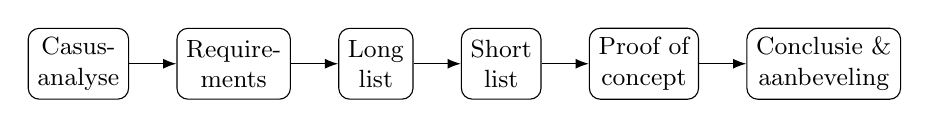
\begin{tikzpicture}[
        node distance=6mm,
        fase/.style={draw, rounded corners, align=center, minimum height=9mm, font=\small}
    ]
        \node[fase] (f1) {Casus-\\analyse};
        \node[fase, right=of f1] (f2) {Require-\\ments};
        \node[fase, right=of f2] (f3) {Long\\list};
        \node[fase, right=of f3] (f4) {Short\\list};
        \node[fase, right=of f4] (f5) {Proof of\\concept};
        \node[fase, right=of f5] (f6) {Conclusie \&\\aanbeveling};
        \draw[-{Latex}] (f1) -- (f2);
        \draw[-{Latex}] (f2) -- (f3);
        \draw[-{Latex}] (f3) -- (f4);
        \draw[-{Latex}] (f4) -- (f5);
        \draw[-{Latex}] (f5) -- (f6);
    \end{tikzpicture}
    \caption{\label{fig:fasen-spec}Fasen van de vergelijkende studie.}
\end{figure*}

\begin{table*}
    \centering
    \small
    \begin{tabular}{p{2.6cm}p{5.4cm}p{5.4cm}p{1.4cm}}
        \toprule
        \textbf{Fase} & \textbf{Onderzoekstechniek} & \textbf{Artefact} & \textbf{Timing} \\
        \midrule
        1. Casusanalyse (DV1) & Semigestructureerd interview met de IT-dienst, documentenanalyse netwerkplan & Beschrijving huidige infrastructuur en filterbeleid, pijnpunten & wk 1-2 \\
        2. Requirements (DV2) & Interviews met belanghebbenden (IT-dienst, directie), MoSCoW-prioritering & Geprioriteerde lijst functionele en niet-functionele requirements & wk 3-4 \\
        3. Long list (DV3, DV4) & Literatuurstudie technische documentatie, niets a priori uitsluiten & Lijst kandidaat-oplossingen met bronvermelding & wk 5-6 \\
        4. Short list (DV4) & Samenvattende tabel requirements $\times$ alternatieven & Gemotiveerde selectie van 2-3 alternatieven & wk 7 \\
        5. Proof of concept (DV5, DV6) & Experiment in gevirtualiseerde testopstelling (VM's die het schoolnetwerk nabootsen), geautomatiseerde metingen, resultaten in CSV, scripts en configuratie in de GitHub-repository & Reproduceerbare testopstelling, meetresultaten (blokkeringsratio, vals-positieven, latency, doorvoer, omzeilbaarheid) & wk 8-11 \\
        6. Conclusie & Analyse en visualisatie meetdata (Python) & Onderbouwde aanbeveling voor College Ten Doorn en resterende hiaten & wk 12 \\
        \bottomrule
    \end{tabular}
    \caption{\label{tab:fasen-spec}Fasen, technieken, artefacten en timing.}
\end{table*}

De criteria in fase 5 zijn bewust meetbaar gedefinieerd: de blokkeringsratio en het aandeel vals-positieven worden bepaald met een vooraf vastgelegde testcorpus van te blokkeren en legitieme domeinen, de prestatie-impact wordt gemeten als extra DNS-latency (ms) en doorvoer (Mbps), en de omzeilbaarheid als het aantal geslaagde bypass-scenario's (DNS-over-HTTPS, alternatieve resolver, VPN). De testopstelling wordt reproduceerbaar en repliceerbaar opgezet: alle configuratie, scripts en ruwe meetdata worden in de projectrepository bijgehouden.

\printbibliography[heading=bibintoc]

\end{document}
